\section{当前工程验收与离线产品结果}
\label{sec:results}
\subsection{完整测试、能力验收和文档范围}
最终完整命令 \cmd{uv run --no-sync pytest} 得到 \textbf{2684 passed in 414.20s}，退出 0，无 failed、skip 或 xfail。启用能力集合为 126 passed in 3.96s，harness-check 为 PASS。126 项是完整套件中的专项集合，不再与 2684 相加。当前收集测试相对原 2562 项增加 122 项，即 4.76\%；这一增量既包括产品契约，也包括共享边界回归，不等于新增 122 种语言语义。

\begin{table}[htbp]\centering\small
\begin{tabularx}{\textwidth}{L{43mm}r r r Y}
\toprule 阶段 & Passed & Failed & 秒 & 解释\\\midrule
核查初始完整套件 & 2560 & 2 & 478.78 & 文档目录与清理夹具失败。\\
修复首次完整套件 & 2682 & 1 & 414.94 & 旧裸票夹具违反全局准入。\\
最终完整套件 & 2684 & 0 & 414.20 & 无 skip/xfail，最终修复源码。\\
最终启用能力集合 & 126 & 0 & 3.96 & 专项检查，包含于完整套件。\\
\bottomrule\end{tabularx}
\caption{真实日志中的工程验收。三次完整运行的用例组成和条件不同，耗时仅作描述。}
\end{table}
\begin{figure}[htbp]\centering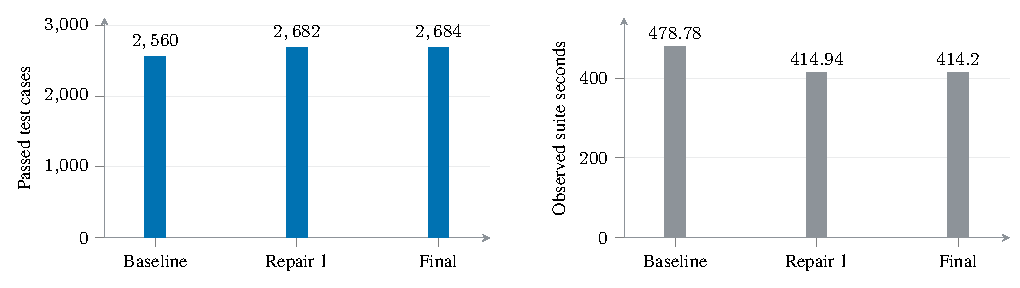
\includegraphics[width=\textwidth]{figures/regression_progress.pdf}
\caption{完整回归的通过数与观测耗时。最终墙钟比初始少 64.58 秒（13.49\%），该差异不能解释为修复带来的因果加速。}\label{fig:regression}
\end{figure}
\source{audit/design_review_20260930/acceptance.json; artifacts/design_review_repair_20260930/final_full_pytest.log}

\subsection{实际 CLI 的状态、分母和证据}
表\ref{tab:cli}逐项报告原验收回执。缺失根和不支持语言在预检阶段阻塞，source\_files=0 表示没有进入有效源码清单统计，不能解释为目标实际有零文件。零候选用例成功完成了一个文件的解析；解析失败用例明确保留一个文件的失败分母。
\begin{table}[htbp]\centering\footnotesize
\begin{tabularx}{\textwidth}{Y L{21mm}c c L{25mm}r}
\toprule 用例 & 运行态 & 源/解析 & 候选/验证/充分 & 性质状态 & 毫秒\\\midrule
\code{literal-mode} & COMPLETED & 1/1 & 1/1/1 & REFUTED & 276.39\\
\code{unknown-mode} & COMPLETED & 1/1 & 1/1/0 & UNKNOWN & 262.45\\
\code{zero-candidates} & COMPLETED & 1/1 & 0/0/0 & -- & 262.43\\
\code{parse-error} & PARTIAL & 1/0 & 0/0/0 & -- & 263.21\\
\code{budget-limited} & PARTIAL & 1/1 & 2/0/0 & UNKNOWN, UNKNOWN & 291.71\\
\code{missing-source} & BLOCKED & 0/0 & 0/0/0 & -- & 256.96\\
\code{unsupported-language} & BLOCKED & 0/0 & 0/0/0 & -- & 272.15\\
\bottomrule\end{tabularx}
\caption{七个真实 CLI 验收用例。每格是单次、自有小源码；0 分母需按预检/清单阶段解释。所有用例均交付 JSON 和 Markdown，模型/目标执行计数均为零。}\label{tab:cli}
\end{table}


\code{literal-mode} 在声明的有界权限位性质上 REFUTED，并不输出全应用 SAFE。\code{unknown-mode} 验证器完成但性质 UNKNOWN，运行仍可 COMPLETED。预算用例含两个候选，在 1800 字节观察上限下两份完整公开证明均未投递：validated=0、sufficient=0、unprocessed=2、公开 observation bytes=0，性质为两个 UNKNOWN。工具调用尝试数为 2，不能写成两次成功验证。其原生产者结果可私有留存，不能用于未交付的强状态。

已有充分证明随后遇到内部失败或取消的保留能力由\emph{另一组}回归验证，该组用例保留先前 REFUTED，停止后续工具并交付局部产物。它不是七个 CLI 中预算用例的结果，两者不能合并叙述。\citep{clireceipt,acceptance}

\begin{figure}[htbp]\centering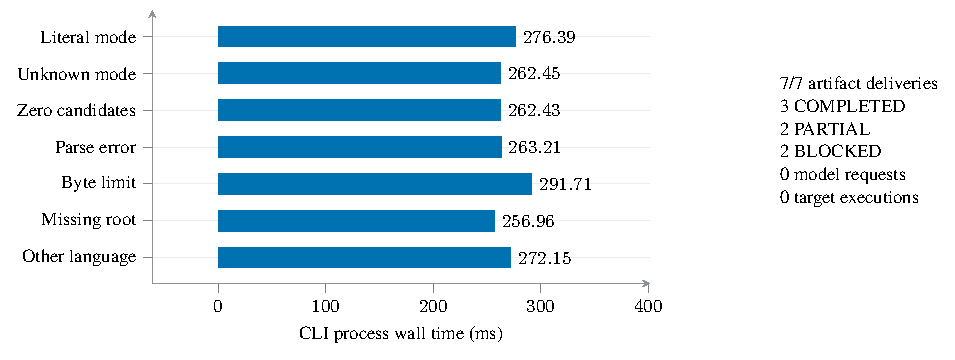
\includegraphics[width=\textwidth]{figures/cli_outcomes.pdf}
\caption{七次真实 console CLI 的运行状态和墙钟。每个用例仅观测一次，极小自有源码且有意包含阻塞与失败路径；不表示真实仓库总体延迟。}\label{fig:cli}
\end{figure}

\subsection{为何必须有多个分母}
这七次运行共有 5 个进入清单的源文件，4 个解析成功、1 个解析失败；发现 4 个候选，2 个验证器完整投递，1 个有充分性质证明，2 个因预算未处理。产物交付 7/7，与性质充分证明 1/4 是不同指标：
\begin{align}
\mathrm{Parsing}_{\mathrm{curated}}&=4/5=80\%,\\
\mathrm{ValidatorCompletion}_{\mathrm{curated}}&=2/4=50\%,\\
\mathrm{SufficientProof}_{\mathrm{curated}}&=1/4=25\%.
\end{align}
候选状态合计 REFUTED 1、UNKNOWN 3，无 SUPPORTED 或 CONFLICT。该计数说明这组路径测试的设计和运行行为，未提供漏洞标签 accuracy、precision、recall 或 FPR。80\%、50\%、25\% 的下降包含有意错误/预算样本，不能据此排列分析器效果优劣。
\begin{figure}[htbp]\centering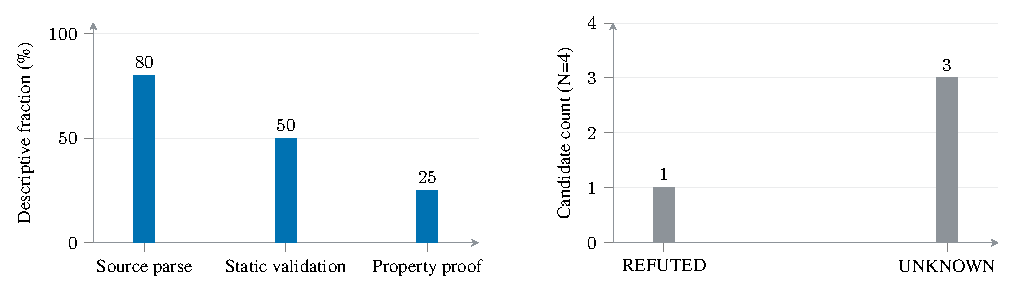
\includegraphics[width=\textwidth]{figures/cli_evidence_denominators.pdf}
\caption{清单、验证完成与充分证明的不同分母，以及四个候选的实际状态。产物成功交付与获得充分性质证明不能互相替代。}
\end{figure}

\subsection{墙钟与成本描述}
七次 console 总墙钟的均值为 \CliMeanMs\ 毫秒，中位数 \CliMedianMs\ 毫秒，范围 \CliMinMs--\CliMaxMs\ 毫秒，样本标准差 \CliStdMs\ 毫秒。每个用例没有重复，未测量并发、冷暖缓存或源码规模曲线，不作生产 SLA 或总体区间推断。内部阶段总计约 11--15 毫秒，与外部 257--292 毫秒不同，主要说明端到端口径包含启动开销；没有单独实验可将差异精确归因到每一模块。

七个用例真实项目模型请求均为 0，physical target executions 均为 0。另一次 transport guard 的 HTTP/socket/live gate 尝试也均为 0。模型费用不应伪造为测量到的 token 单价成本；静态 profile 的 reported\_tokens 未调用 provider，按结果契约保留相应不可用含义。文档写作和内部审阅不纳入项目历史模型实验账本。\citep{transportguard,clireceipt}

\subsection{验收矩阵和门槛状态}
A01--A34 共 34 项，启用静态 profile 的 31 条必需项全通过；A27--A29 是条件 scratch/native 能力，仍未启用/未运行。若将分母写成 34 而宣称全部通过，会掩盖条件范围；若删除三项，又丢失扩展义务。正确当前描述是 \textbf{31/31 必需通过 + 3 条件未提供}。

\begin{figure}[htbp]\centering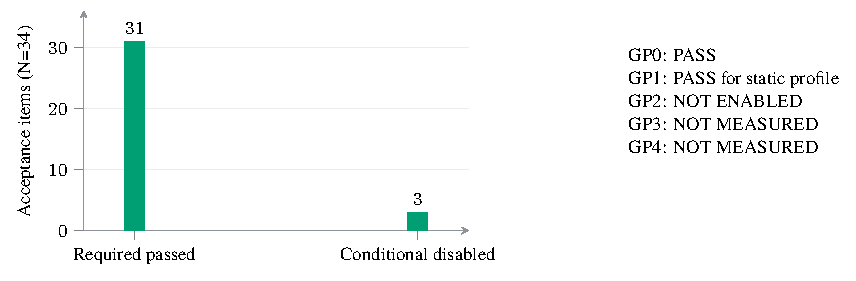
\includegraphics[width=\textwidth]{figures/acceptance_gates.pdf}
\caption{当前验收矩阵与产品门槛。GP0/GP1 通过限于默认静态路径；GP2 未启用，GP3/GP4 尚未测量。附录保留全部 34 项。}\label{fig:acceptance}
\end{figure}

GP0/GP1 只验收离线产物和启用静态控制；GP2 是未启用的条件执行能力。GP3 的人工价值与 GP4 的模型净增量仍未测量，前瞻方案见第\ref{sec:limits}节。
